Die hier zu entwickelnde Anwendung dient zum Anlegen und Verwalten von Aufgaben der Nutzer*innen. Somit löst sie die sogenannte, analoge \textit{To-Do-Liste} ab. Dabei hat die Anwendung (und somit auch die Studienarbeit) keinen Anspruch auf Innovationsdarbierung. Die Begründung der dieses speziellen Entwicklungsbeispiels liegt darin, dass eine To-Do-Listen-Anwendung ein großes Spektrum von Funktionen abbilden kann. Dieses Spektrum reicht von grundlegenden Funktionen (bspw. dem bloßen Anlegen von Aufgaben) bis zu komplexeren Inhalten (bspw. automatischen Push-Notifications über unerledigte oder überfällige Aufgaben). Diese design- und architekturbedingenden Entscheidungen werden im Folgenden definiert und näher beschrieben.

Die Beschreibung der Architektur einer zu entwickelnden Applikation ist eine maßgebende Disziplin im Software-Engineering-Prozess. Dieser Prozess geschieht im Regelfall vor Beginn der Implementierung und ermöglicht, bezogen auf den Umfang dieser Studienarbeit, die Vergleichbarkeit der Applikation hinsichtlich der relevanten Entwicklungsplattformen. Der Umfang sämtlicher Software-Engineering-Prozesse wird grundsätzlich in großen Entwicklerteams praktiziert. Diese gehen der Entwicklung meist komplexer und skalierbarer Anwendungen nach. Im Vergleich dazu ist die hier zu entwickelnde Mobilanwendung lediglich Mittel zum Zweck für die Beantwortung der Forschungsfrage. Das Entwicklungsteam der To-Do-Anwendung besteht aus zwei Personen, welche sich im Rahmen dieser Arbeit autark mit unterschiedlichen Entwicklungsplattformen beschäftigen. 

Dies sorgt dafür, dass sich lediglich eine abgespeckte Form des Software-Engineering auf dieses Projekt anwenden lässt. Konkret bedeutet dies, dass zum Einen keine spezifischen Aussagen über den Software-Prozess bzw. über das Entwicklungsmodell (Wasserfall-Modell, iteratives Modell, etc.) gemacht werden. Dies würde sich hinsichtlich des verhältnismäßig geringen Entwicklungs- und Wartungsaufwands der App kontraproduktiv auf die Zielorientierung auswirken. Umso wichtiger ist die Definition funktionaler sowie nicht-funktionaler Anforderungen, welche daraufhin näher erläutert und spezifiziert werden. Auch die Interaktion zwischen Nutzer*in und Anwendung muss für eine vergleichende Entwicklung definiert werden. Die zeitlichen und komponentenabhängigen Abläufe innerhalb der App gehören ebenfalls zu den Bestandteilen der Architektur. Letztere beiden Punkte werden im Rahmen des sog. \textit{Systems Modelling} definiert. Darüber hinaus werden auch optische Aspekte und Verhaltensweisen des \ac{ui} abgegrenzt.

\section{Anforderungsdefinition}
Die Funktionalität der Anwendung wird zunächst über die Anforderungsdefinition näher beschrieben. Diese kann auf allgemeine Funktionsweisen der App (nicht-funktionale Anforderungen), sowie auf spezifische, technische Charakteristika abgegrenzter Bereiche der Anwendung (funktionale Anforderungen). Grundsätzlich gilt es, nicht-funktionale Anforderungen im Laufe der Anforderungsdefinition in meist mehrere funktionale Anforderungen zu überführen, da diese qualifizierbarer sowie quantifizierbarer Natur sind und somit ebenfalls für eine bessere Vergleichbarkeit der zu entstehenden Anwendungen beitragen könnten.

\subsection{Nicht-Funktionale Anforderungen}
Die folgenden nicht-funktionalen Anforderungen beziehen sich auf Teile der Anwendung, welche jedoch abstrakter Natur sind, weswegen sie zunächst zu nicht-funktionalen Anforderungen gezählt werden müssen. Aufgrund der Formulierung werden diese Anforderungen auch als \textit{Nutzeranforderungen} (engl. \textit{User Requirements}) bezeichnet und stehen den spezifischeren, technisch versierteren \textit{Systemanforderungen} (engl. \textit{System Requirements}) gegenüber.
\begin{description}
    \item[Anlegen, Auflisten, Bearbeiten und Löschen von Aufgaben] Die Anwendung ermöglicht es, Aufgaben hinzuzufügen. Die hinzugefügten Aufgaben werden aufgelistet. Bei Bedarf soll der Inhalt der Aufgabe nachträglich abgeändert werden können. Ebenfalls ist es möglich, die Aufgabe aus der Ansicht innerhalb der Anwendung zu entfernen.
    \item[Aufgaben bestehen nach Neustart der Anwendung bei] Wird die Applikation (gewollt und ungewollt) neu gestartet, bildet sie nach Neustart dieselben Aufgaben und Einstellungen wie zuvor ab.
    \item[Priorisierung der Aufgaben möglich] Bei Bedarf ist es möglich, einer bestimmten Aufgabe einen gesonderten Stellenwert zuzuweisen.
    \item[Benachrichtigungen über nicht-erledigte und überfällige Aufgaben] Der*die Nutzer*in wird unabhängig vom Status der Applikation oder des Smartphones (d.h. geöffnet, im Hintergrund oder geschlossen bzw. gesperrt oder entsperrt) über nicht-erledigte und überfällige Aufgaben benachrichtigt.
\end{description}
Neben dieser Art der nicht-funktionalen Anforderungen koexisitieren jene, welche zwar ebenfalls abstrakt und allgemein gehalten sind, jedoch keinen Bedarf resp. keine Möglichkeit zur weiteren Spezifizierung an dieser Stelle des Prozesses aufweisen.
\begin{description}
    \item[Bereitstellung der Anwendung für mehrere Plattformen] Die Anwendung ist nicht nur auf einer Plattform verfügbar, sondern kann auf Geräten unterschiedlicher Betriebssysteme installiert und verwendet werden.
    \item[Aussehen und Verhalten sind deckungsgleich] Unabhängig davon, welche Plattform genutzt wird, ist die Interaktion zwischen dem*der Nutzer*in und der Anwendung annähernd identisch. Davon ausgenommen sind Aspekte, welche auf der entsprechenden Plattform nicht oder nur mit unverhältnismäßigem Aufwand erreicht werden können.
    \item[zeiteffizienter Entwicklungsprozess] Um auch einen entwicklungstechnischen Vergleich ziehen zu können, soll die Anwendung in einer dem Projekt angemessenen Zeit vollständig entwickelt werden können.
\end{description}
Die Problematik nicht-funktionaler Anforderungen im Bezug auf realistisch zu betrachtende Entwicklungsprojekte kann hier interpretiert werden. Vor allem bei eher unerfahrenen Entwicklern (zu welchen sich das Entwicklerteam dieses Projektes zu zählen erlaubt) sind bestimmte Tendenzen unklar. Dazu gehören bspw. das Bewusstsein über die Realisierbarkeit bestimmter Komponenten sowie die zeitliche Aufwandseinschätzung. Diese Störfaktoren werden im Laufe der Arbeit versucht, entkräftet zu werden und sind in die Evaluation der Forschungsfrage kritisch einzubeziehen.

\subsection{Funktionale Anforderungen}
Nichtsdestotrotz ist die Spezifizierung der in Sektion 3.1.1 eingangs definierten nicht-funtionalen Anforderungen noch ausstehend. Zur Unterstützung der Lesbarkeit werden diese in Reihenfolge der nicht-funktionalen Anforderungen abgehandelt.

\begin{description}
    \item[Bereitstellung klassischer \acs{crud}-Operationen] Sog. \textit{\ac{crud}}-Operationen greifen auf das Datenmodell der Anwendung zu. Diese erlauben die Manipulation der Daten auf Basis der gewünschten Operation. Diese Operationen sind unabhängig voneinander zu definieren und sinnvoll in den Verwendungsprozess der App einzubauen. Man spricht hier auch von sog. \ac{crud}-\textit{Endpoints}, welche vereinfacht als statische Funktionen beschrieben werden können.
    \item[Listendarstellung] Die Aufgaben sollen grundsätzlich in einer sortierten Liste dargestellt werden. Die Liste besteht aus individuellen Elementen, welche jeweils eine Aufgabe darstellen. Jene \ac{crud}-Operationen, welche speziell auf eine bestimmte Aufgabe angewandt werden sollen, finden ihre Aktivierung ebenfalls über ihre entsprechenden Elemente.
    \item[Bereitstellung eines Persistent Services] Bei Ausführen der zuvor definierten \ac{crud}-Operationen werden die Daten nicht nur in den flüchtigen Arbeitsspeicher des Smartphones geschrieben, sondern zugleich auch auf einen der Applikation zugewiesenen Festspeicher. Diese idealisierte Datenbank gleicht dem Datenmodell für die \ac{crud}-Operationen und wird somit bei jeder Ausführung dieser aktualisiert bzw. beansprucht.
    \item[Definition einer Hierarchie für Aufgaben] Eine hierarchische Struktur der Daten soll ermöglichen, bestimmte Aufgaben seitens der Anwendung anders zu behandeln als andere. Durch das Setzen eines sog. \textit{Flags} können die Aufgaben entsprechend der Hierarchiestruktur bestimmte Zustände übergeben bekommen, konkret eine hervorgehobene optische Darstellung innerhalb der \ac{ui} sowie die Präsentation an Anfang der Liste (Eingriff in die Sortierung der Aufgaben)
\end{description}

Streng genommen sind funktionale Anforderungen sehr granulär zu definieren. Da es sich hier jedoch um eine wissenschaftliche Arbeit handelt, und nicht um eine Entwicklerdokumentation, wird auf kleinste Genauigkeiten verzichtet. Viel eher soll die nächste Sektion die genaue, weiterhin plattformunabhängige Umsetzung dieser Anforderungen erläutern, welche als Maßgabe für die spätere Entwicklung der Applikation dienen soll. 

\section{Funktionen}

Die Anwendung unterstützt klassische \ac{crud}
CRUD\\
offline cache\\

\section{Oberfläche (\ac{ui})}

\subsection{Elemente}
-Todo Listen eintrag
    -Flag important
    -checkbox
    -edit Methode
    -delete
-Input Methode

\begin{figure}[h]
        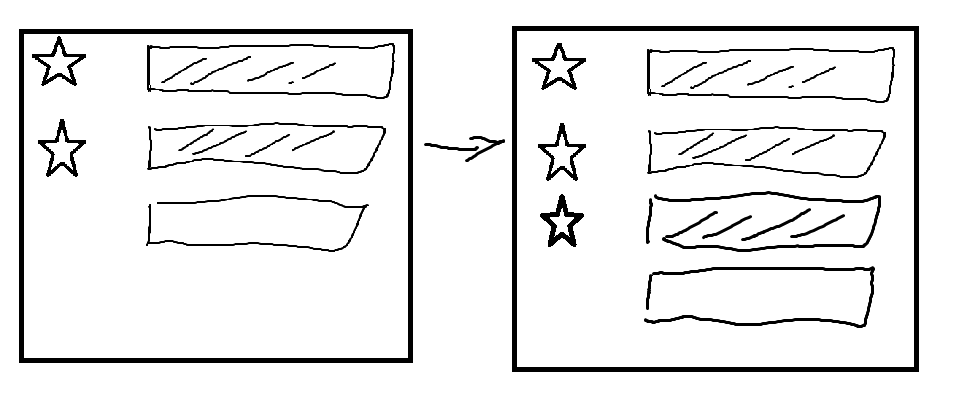
\includegraphics[width=\linewidth]{img/sketch_insert.png}
        \centering
        \caption{Verhalten beim Einfügen}
        \label{fig:inserttodo}
\end{figure}

\subsection{Größen}
\begin{figure}[h]
        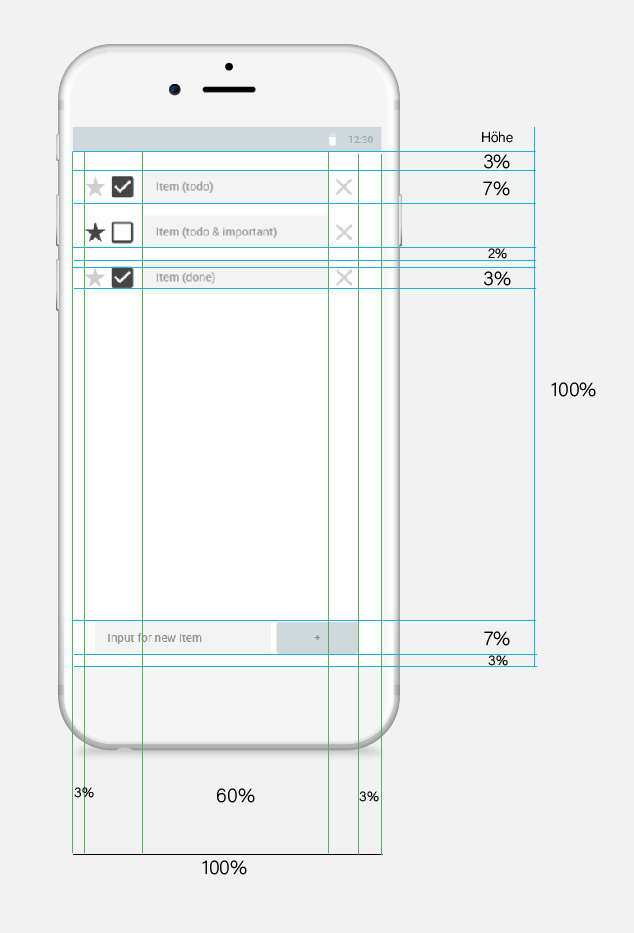
\includegraphics[scale=0.5]{img/Wireframe_dimensions.jpg}
        \centering
        \caption{Größen}
        \label{fig:dimensions}
\end{figure}

\subsection{Farben}

Um die Anpassungsmöglichkeiten von nativen Apps und PWA zu evaluieren, werden in Tabelle \ref{tab:farbtabelle} Farben für einzelne Elemente des User Interface festgelegt.

\begin{table}
  \centering
    \begin{tabular}{ |c|c|c|}
     \hline
    \textbf{Bezeichnung} & \textbf{HEX-Code} & \textbf{Beispiel}\\
    \hline
    
    
    \hline
    \multicolumn{3}{|c|}{\textbf{Allgemeines}}\\
     \hline
    Hintergrund & \texttt{\#F2F2F2} &\cellcolor[HTML]{F2F2F2}\\
        \hline
         Schriftfarbe & \texttt{\#8C8C8C} &\cellcolor[HTML]{8C8C8C}\\
     \hline
     
     
      \hline
    \multicolumn{3}{|c|}{\textbf{Bedienelemente}}\\
     \hline
      Hintergrund für inaktive Bedienelemente & \texttt{\#CECECE} &\cellcolor[HTML]{CECECE}\\
     \hline
    Checkbox (checked) Hintergrund & \texttt{\#1A66FF} &\cellcolor[HTML]{1A66FF}\\
    \hline
     Schriftfarbe der Checkbox (checked) & \texttt{\#FFFFFF} &\cellcolor[HTML]{FFFFFF}\\
     \hline
    \end{tabular}
  \caption{Farbtabelle} \label{tab:farbtabelle}
\end{table}


\subsection{Aussehen/Design}



\begin{figure}[h]
        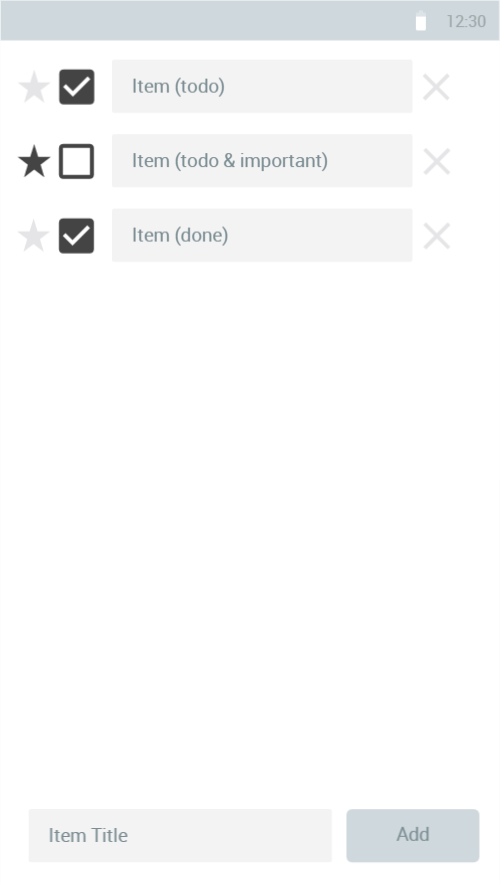
\includegraphics[scale=0.5]{img/wireframe.png}
        \centering
        \caption{Wireframe}
        \label{fig:wireframe}
\end{figure}







\section{Komponenten}
\begin{description}
    \item \textbf{App Container}\\
    Das unterste UI-Element der Anwendung wird im Folgenden als App Container bezeichnet, da es aufgrund der verschiedenen Technologien keine einheitliche Bezeichnung dafür gibt. Der App Container ist bei der PWA das \texttt{body} Element des HTML und bei der nativen iOS App ein \texttt{View} Element.
    
    \textbf{Besonderes:} Ist der Inhalt des App Containers größer, als der Bildschirm, wird in vertikale Richtung gescrollt. Es gibt kein horizontales Scrolling, stattdessen müssen sich alle anderen Elemente automatisch anpassen.

    \item \textbf{Todoliste}\\
    Der Kern der Anwendung ist eine Liste, die einzelne Todos enthält. Neue Todos werden stets unten an die Liste angefügt.
    
    \textbf{Besonderes:} Es gibt genau eine Todoliste. Sie kann nicht gelöscht werden und enthält mindestens ein (leeres) Todo.
    
    \item \textbf{Todo (Listeneintrag)}\\
    Ein Todo ist ein Listenelement der Todoliste. Dieses besteht aus einem editierbaren Textfeld. Seitlich des Textfelds befinden sich Buttons zum Entfernen des Eintrags und zum Markieren des Eintrags als "wichtig".
    
    Das Todo hat links neben dem Eingabefeld eine Checkbox. Bis zum "check" durch den Nutzer ist die Checkbox nicht markiert.
    
    \textbf{Besonderes:} Wenn der Inhalt eines bestehenden Todos gelöscht wird, bleibt es bestehen und wird nicht automatisch entfernt.
    
    \item \textbf{Eingabemöglichkeit}\\
    Damit der Nutzer neue Todos eintragen kann, wird ein Eingabefeld benötigt. Das Eingabefeld ist idealerweise in die Todoliste integriert. Für den Nutzer soll stets ein Eingabefeld unter der Todoliste sichtbar sein.
    Da bereits die Todoliste aus einzelnen Eingabefeldern besteht, muss diese während der Eingabe eines neuen Elements nur um ein neues leeres Listenelement erweitert werden.
    
    \textbf{Besonderes:} Es werden keine leeren Todos eingefügt. Ein Todo muss mindestens ein Zeichen enthalten.
\end{description}

\section{Designentscheidungen PWA}
Seit 2014 bis heute ist JavaScript die häufigste Sprache auf GitHub. Das stärker typisierte TypeScript gehört zu den am schnellsten wachsenden Sprachen \cite{OctoverseGitHubStatistics}. Um diese Arbeit zukunftsgewandt zu evaluieren, werden deshalb das bereits beschriebene Angular-Framework verwendet, dass TypeScript (transpilierter zu JavaScript) und die Node.js Laufzeitumgebung nutzt. Nicht zuletzt ist auch der Große Beitrag von Google (als Mobilgerätehersteller und Betriebssystementwickler von Android) zum Angular-Projekt ein Grund, die PWA in Form einer Angular Anwendung zu realisieren.


